\chapter{Wykład 3. Środowisko zarządzania projektami w przedsiębiorstwie}

\section{Strategia firmy}
% strona 8

\subsection*{Wizja}

Wizją naszego przedsiębiorstwa jest stworzenie systemów wspierających zarządzanie projektami informatycznymi.

\subsection*{Misja}

Nasza firma dąży do tego, aby być najlepszym pod względem jakości i niezawodności dostawcą oprogramowania do zarządzania projektami informatycznymi na rynku.

\subsection*{Cele strategiczne}

Plan dwuletni naszego przedsiębiorstwa zakłada:
\begin{itemize}
\item stworzenie sztandarowego produktu firmy, który zapewni rozpoznawalność marki oraz stały dochód na poziomie 200 000 zł miesięcznie,
\item wypuszczenie na rynek dwóch kolejnych produktów,
\item osiągnięcie sprzedaży na poziomie 50 licencji na kwartał,
\item ekspansja działalności firmy na rynki czeski i słowacki.
\end{itemize}

\subsection*{Zasady (Wartości)}

\begin{itemize}
\item Dobre traktowanie pracowników
\item Najwyższa jakość produktów
\item Bezstronność
\item Niezależność od innych przedsiębiorstw
\end{itemize}

% ===========================================================================

\section{Strategia rozwoju firmy}
% strona 14

Nasza firma w swojej działalności stawia na innowacyjność. Działalność operacyjna obejmuje tworzenie oprogramowania wspierającego zarządzanie projektami w przedsiębiorstwach. Jako firma wyznaczamy nowe kierunki działania i eksperymentujemy z nowymi technologiami. Staramy się zrozumieć potrzeby naszego Klienta. Współpraca biznesowa z Klientem jest bardzo ważnym czynnikiem rozwoju firmy. 
Jako pracodawca staramy się inwestować w młody i ambitny zespół. Potrzeby naszego pracownika są dla nas bardzo ważne, dlatego szczególną uwagę zwracamy na środowisko pracy, stałe zatrudnienie oraz opiekę socjalną pracownika. Wierzymy, że zadowolony pracownik to wydajny pracownik, dzięki, któremu możliwy jest sukces firmy.  

\textbf{Powiązania strategii ze szkołami zarządzania strategicznego:}

\textit{Szkoła zasobów i kompetencji} – nacisk na dbanie o pracownika i przeświadczenie, że praca jednostki składa się na sukces całego przedsięwzięcia.

\textit{Szkoła planistyczna} – strategia stworzona na bazie analizy SWOT.


% ===========================================================================

\section{Sieć zależności korzyści}
% strona 37

\begin{figure}[!h]
\centering
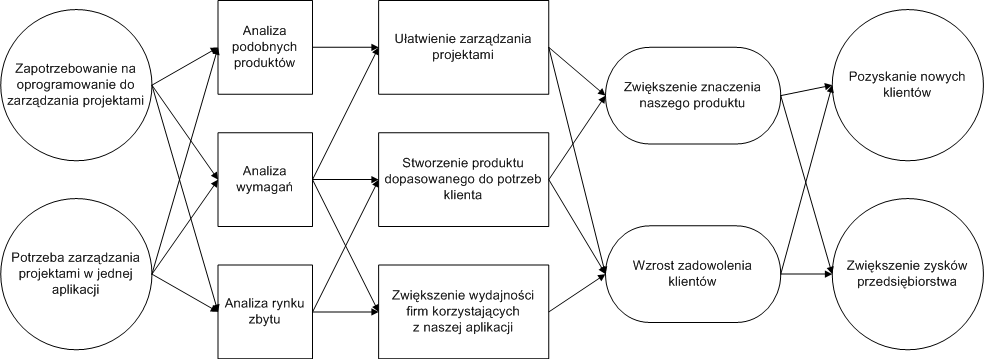
\includegraphics[width=\textwidth]{siecZaleznosciKorzysci}
\caption{Sieć zależności korzyści}
\label{fig:siecZaleznosciKorzysci}
\end{figure}

%\clearpage

% ===========================================================================

\section{Zarządzanie portfelem projektów}
% strona 47

Głównym celem zarządzania portfelem projektów jest określenie priorytetów i składowych portfela, przy jednoczesnym upewnieniu się, że są zgodne z celami strategicznymi organizacji.

Zarządzanie portfelem projektów składa się z:
\begin{itemize}
\item definicji portfeli wewnątrz organizacji
\item podzielenia projektów na kategorie
\item identyfikacji i ocenie grup projektów i ich dopasowania do celów organizacji
\item nadania priorytetów
\item pozyskania informacji o zasobach i ich przydzielenia
\item porównania potrzebnych zasobów i dostępnych możliwości
\item określenie ryzyka w projektach i sposobów jego łagodzenia
\end{itemize}

Klasyfikacja projektów w portfelu:
\begin{itemize}
\item macierz BCG
\begin{itemize}
\item dojne krowy, gwiazdy, znaki zapytania, kule u nogi
\item skupienie się na dojnych krowach i gwiazdach
\end{itemize}
\item macierz atrakcyjności projektów
\begin{itemize}
\item policzenie punktacji dla każdego projektu
\item skupienie się na tych lepiej punktowanych
\end{itemize}
\end{itemize}

Inne ważne kryteria wyboru projektów:
\begin{itemize}
\item dochodowość
\item szacowany udział w rynku
\item prawdopodobieństwo osiągnięcia sukcesu
\end{itemize}

% ===========================================================================

\section{Czynniki środowiskowe}
% strona 78

\subsection*{Wewnętrzne}

\begin{itemize}
\item Struktura organizacyjna,
\item Kultura i styl organizacyjny,
\item Procesy, procedury i rozwiązania,
\item Etyka pracy i godziny pracy,
\item Lokalizacja (początkowo jedno biuro, po rozszerzeniu działalności nastąpi rozproszenie na kilka miejsc),
\item Infrastruktura,
\item Oprogramowanie i narzędzia pracy (do zarządzania projektami, jak i do ich tworzenia),
\item Polityka administrowania personelem,
\item Nastawienie wobec ryzyka,
\item Dostępność oraz poziom kompetencji zasobów,
\item System weryfikacji pracy.
\end{itemize}

\subsection*{Związane z partnerami}

\begin{itemize}
\item Kultura organizacyjna,
\item Nastawienie wobec ryzyka,
\item Narzędzia stosowane przez partnerów.
\end{itemize}

\subsection*{Zewnętrzne}

\begin{itemize}
\item Standardy przemysłowe i rządowe regulacje,
\item Uwarunkowania rynkowe.
\end{itemize}

